\documentclass[11pt]{beamer}
\usetheme{Madrid}
\usefonttheme{serif}

\usepackage[utf8]{inputenc}       % Encoding
\usepackage[english]{babel}       % Language
\usepackage[T1]{fontenc}          % Font encoding

\usepackage{amsmath, amsfonts, amssymb} % Math packages
\usepackage{graphicx}
\usepackage{xcolor}
\usepackage{colortbl}
\usepackage{array}
\usepackage{subcaption}

\usepackage{tikz}
\usepackage{tikz-uml}
\usetikzlibrary{arrows.meta, positioning, calc}
\usepackage{blkarray}
\usepackage{pgfplots}
\pgfplotsset{compat=1.18}

%Tabular
\usepackage{tabularx}
\usepackage{multirow}
\usepackage[table]{xcolor}
\usepackage{enumitem}
\usepackage{booktabs}
\usepackage{arydshln}

% Code formatting
\usepackage{minted}
\usepackage{adjustbox}
\usepackage[ruled,vlined]{algorithm2e}
\SetKwProg{While}{while}{}{}
\SetKwProg{For}{for}{}{}
\SetKwProg{Function}{function}{}{}

% Custom math operators
\DeclareMathOperator{\sen}{sen}
\DeclareMathOperator{\tg}{tg}

% Numbered captions in figures/tables
\setbeamertemplate{caption}[numbered]

% Metadata
\author[Mathys Vinatier]{Mathys Vinatier}
\title{PPO Market Bot}
\setbeamercovered{transparent}
\setbeamertemplate{navigation symbols}{}
\logo{\includegraphics[scale=.05]{../img/logoSNU.png}}
\institute[]{Seoul National University}
\date{\today}

% Bibliography
\usepackage{biblatex} 
\addbibresource{../references.bib}
\usepackage{csquotes}

%Glossary
\usepackage[acronym]{glossaries}
\makeglossaries
% glossary.tex (no preamble commands here)

\newacronym{PPO}{PPO}{Proximal Policy Optimizer}

\newacronym{ALS}{ALS}{Autocovariance Least-Squares}

\newacronym{FKF}{FKF}{Field Kalman Filter}

\newacronym{OKF}{OKF}{Optimized Kalman Filter}

\newacronym{NN}{NN}{Neural Network}

\newacronym{RNN}{RNN}{Recursive Neural Network}

\newacronym{LSTM}{LSTM}{Long Short-Term Memory}

\newacronym{MB}{MB}{Model Based}

\newacronym{KF}{KF}{Kalman Filter}

\newacronym{EKF}{EKF}{Extended Kalman Filter}

\newacronym{DD}{DD}{Data Driven}

\newacronym{KG}{KG}{Kalman Gain}

\newacronym{SS}{SS}{State Space}

\newacronym{MSE}{MSE}{Mean Square Error}

\newacronym{SPD}{SPD}{Symmetric Positive Definite}

\newacronym{WFA}{WFA}{Walk Forward Analysis}

\newacronym{TRPO}{TRPO}{Trust Region Policy Optimization}

\newacronym{LMA}{LMA}{Logarithmic Movement Average}

\newacronym{RL}{RL}{Reinforcement Learning}

\newacronym{MDP}{MDP}{Markov Decision Process}

\newacronym{API}{API}{Approximate Policy Iteration}

\newacronym{LR}{LR}{Logistic Regression}

\newglossaryentry{KalmanNet}{
    name={KalmanNet},
    description={Neural network-based model that integrates Kalman filtering techniques for improved state estimation in dynamic systems.}
}


\begin{document}

\begin{frame}
    \titlepage
\end{frame}

\begin{frame}{PPO Agent}
    \textbf{Actor-Critic Layouts}
    \hfill
    \begin{figure}[!ht]
        \centering
        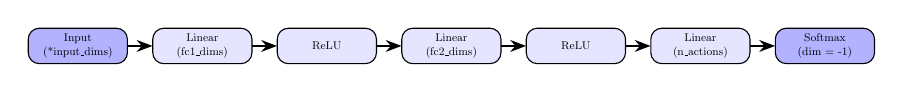
\begin{tikzpicture}[
            scale=0.45,
            transform shape,
            node distance=0.7cm,
            box/.style={
                draw,
                rounded corners,
                minimum width=2.8cm,
                minimum height=1cm,
                align=center,
                font=\small,
                fill=blue!10
            },
            arrow/.style={
                -{Stealth[length=2mm]},
                thick
            }
        ]

            % Nodes
            \node[box, fill=blue!30] (input) {Input \\ (*input\_dims)};
            \node[box, right=of input] (fc1) {Linear \\ (fc1\_dims)};
            \node[box, right=of fc1] (relu1) {ReLU};
            \node[box, right=of relu1] (fc2) {Linear \\ (fc2\_dims)};
            \node[box, right=of fc2] (relu2) {ReLU};
            \node[box, right=of relu2] (fc3) {Linear \\ (n\_actions)};
            \node[box, fill=blue!30, right=of fc3] (softmax) {Softmax \\ (dim = -1)};

            % Connectors
            \draw[arrow] (input) -- (fc1);
            \draw[arrow] (fc1) -- (relu1);
            \draw[arrow] (relu1) -- (fc2);
            \draw[arrow] (fc2) -- (relu2);
            \draw[arrow] (relu2) -- (fc3);
            \draw[arrow] (fc3) -- (softmax);

        \end{tikzpicture}
        \caption{Actor network architecture (Softmax output)}
    \end{figure}
    \hfill
    \begin{figure}[!ht]
        \centering
        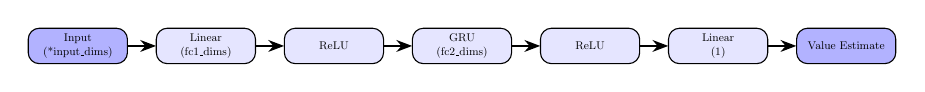
\begin{tikzpicture}[
            scale=0.45,
            transform shape,
            node distance=0.8cm,
            box/.style={
                draw,
                rounded corners,
                minimum width=2.8cm,
                minimum height=1cm,
                align=center,
                font=\small,
                fill=blue!10
            },
            arrow/.style={
                -{Stealth[length=2mm]},
                thick
            }
        ]

            % Nodes
            \node[box, fill=blue!30] (input) {Input \\ (*input\_dims)};
            \node[box, right=of input] (fc1) {Linear \\ (fc1\_dims)};
            \node[box, right=of fc1] (relu1) {ReLU};
            \node[box, right=of relu1] (fc2) {GRU \\ (fc2\_dims)};
            \node[box, right=of fc2] (relu2) {ReLU};
            \node[box, right=of relu2] (fc3) {Linear \\ (1)};
            \node[box, fill=blue!30, right=of fc3] (out) {Value Estimate};

            % Connectors
            \draw[arrow] (input) -- (fc1);
            \draw[arrow] (fc1) -- (relu1);
            \draw[arrow] (relu1) -- (fc2);
            \draw[arrow] (fc2) -- (relu2);
            \draw[arrow] (relu2) -- (fc3);
            \draw[arrow] (fc3) -- (out);

        \end{tikzpicture}
        \caption{Critic network architecture (GRU layout)}
    \end{figure}
    \hfill
\end{frame}

\begin{frame}{PPO Agent}
    \textbf{Training the Agent}

    \centering
    \resizebox{!}{0.4\textheight}{%
    \begin{algorithm}[H]
    \caption{PPO Agent Training Loop}
    \KwIn{$env$, $n\_games$, $N$, $batch\_size$, $\alpha$, $n\_epochs$}
    \KwOut{Trained PPO agent, episode rewards}

    Initialize PPO\_agent;

    \For{$i \leftarrow 1$ \KwTo $n\_games$}{
        $s \leftarrow env.reset()$\;
        $done \leftarrow \text{False}$\;
        $score \leftarrow 0$\;
        
        \While{$done = \text{False}$}{
            $A_{valid} \leftarrow env.get\_valid\_actions()$\;
            $(a, \text{probs}, v) \leftarrow agent.choose\_action(s, A_{valid})$\;
            $(s', r, done, info) \leftarrow env.step(a)$\;
            
            $score \leftarrow score + r$\;
            $n\_steps \leftarrow n\_steps + 1$\;
            $agent.remember(s, a, \text{probs}, v, r, done)$\;
            
            \If{$n\_steps \bmod N = 0$}{
                $agent.learn()$\;
                $learn\_iters \leftarrow learn\_iters + 1$\;
            }
        }
    }
    \Return trained agent\;
    \end{algorithm}
    }
\end{frame}

\begin{frame}{PPO Agent}
    \textbf{First Result after 500 episodes training}
    \begin{figure}[!ht]
        \centering
        \includegraphics[width=.9\textwidth]{../img/PPO/plot_ppo_first_try.png}
        \caption{First ouput for PPO agent}
    \end{figure}

\end{frame}

\begin{frame}{Trade Station Server}
    \begin{figure}[!ht]
        \centering
        \includegraphics[width=.7\textwidth]{../img/diagram/Server_architecture.drawio.png}
        \caption{Architecture of the Service}
    \end{figure}
\end{frame}

\begin{frame}{Trade Station Server}
    \begin{figure}[!ht]
        \centering
        \includegraphics[width=\textwidth]{../img/diagram/UML_service.drawio.png}
        \caption{UML of the Service}
    \end{figure}
\end{frame}

\begin{frame}
    \centering
    \vspace{2cm}
    {\LARGE Thank You}
\end{frame}

\end{document}
